\section{Water}
The water is basically a squared plane (built in the same way of the flat terrain). Each cell has a water plane that will be visible only if some vertex of the cell has an height < of the water.

\begin{figure}[hbt!]
	\centering
	\subfloat[\centering Plane.]{{
\includegraphics[width=6.3cm]{images/Water.png}}}%
	\qquad
	\subfloat[\centering Vertices, indices and faces.]{{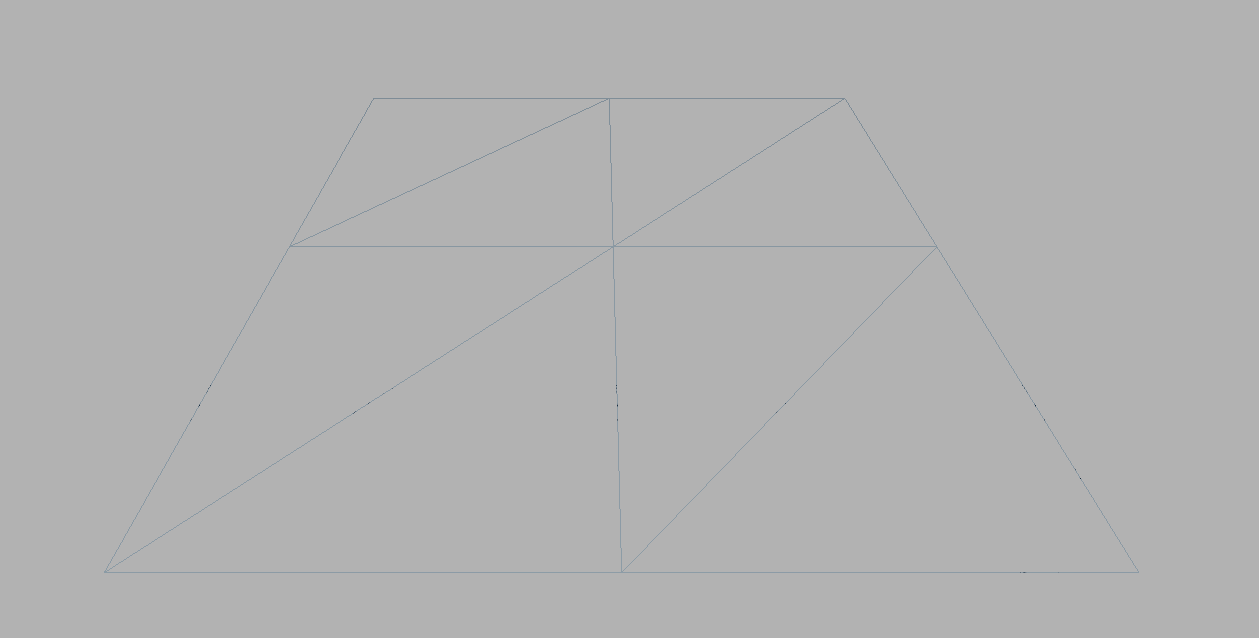
\includegraphics[width=6.3cm]{images/WaterNoVert.png} }}%
	\caption{}
\end{figure}

\section{Reflection and refraction}
After creating the plane, the first thing I implemented was the reflaction and the refraction on the plane.

\subsubsection{Frame buffer objects}
The frame buffer is used to render our scene with all the information from the different buffers, such as color and depth. You can create your own frame buffer object to render the scene and save it in a texture. In particular, every time we render the scene in our frame buffer, we will update our 2D texture. This is exactly what we need because we need a texture to project inside the plane.
I'll quickly explain how I created the class for the frame buffer object (Full code in \textbf{waterFrameBuffer.h}).

\newpage

\noindent
First I defined a method to create the frame buffer using some OpenGL function.

\begin{figure}[hbt!]
	\centering
	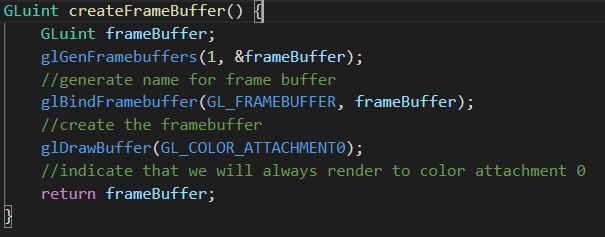
\includegraphics[width= 1
	\textwidth]{images/FBO1.png}
	\caption{Method for the creation of the frame buffer.}
\end{figure} 

\noindent
So I defined the two methods of creating texture attachment, one for colour and one for depth attachment. They are just a simple generation of a texture with a new "glFramebufferTexture" statement. (I only insert the screenshot of the attached colour since they are pretty much the same).

\begin{figure}[hbt!]
	\centering
	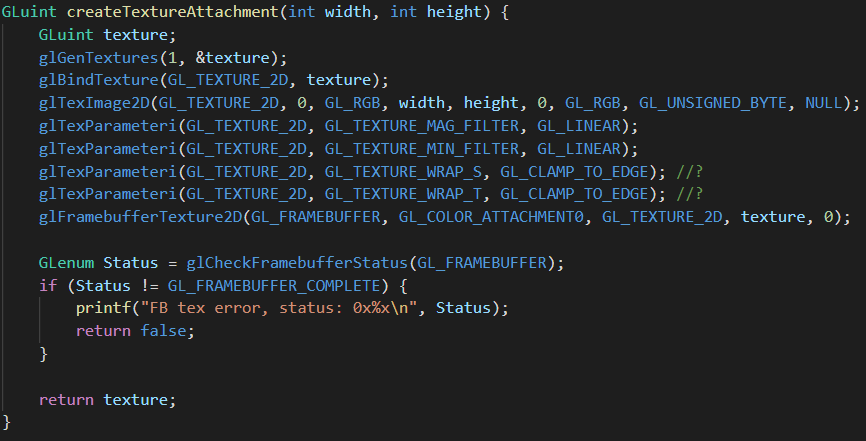
\includegraphics[width= 0.9
	\textwidth]{images/FBO2.png}
	\caption{Method for the creation of the texture.}
\end{figure} 

Last I defined a method to create the depth buffer. 

\begin{figure}[hbt!]
	\centering
	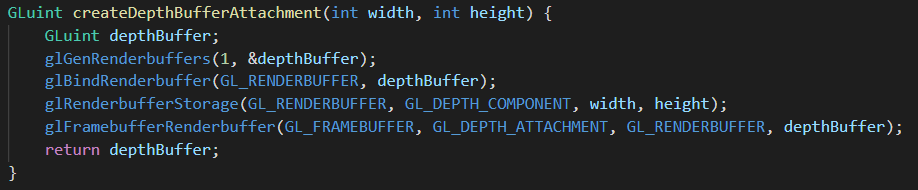
\includegraphics[width= 1
	\textwidth]{images/FBO4.png}
	\caption{Method for the creation of depth buffer.}
\end{figure} 

\noindent
Finally I created two methods, one to bind the frame buffer and one to unbind it so that I can switch from the normal frame buffer to the one created by me. I stored two frame buffers in this class, one for reflection and one for refraction. Basically I'll render the scene and create my own texture that will be used by the main render to apply it to the water.

\subsection{Clipping plane}
For both refraction and reflection textures, you don't need to render the whole scene. Actually I need the one above the surface for the reflection and the one under the water for refraction. So I defined the clipping plane which allowed me to render only a part of the scene and obviously it is positioned at the same level of the water. \\
After enabling a clipping plane (\textbf{glEnable(GL\textunderscore CLIP \textunderscore DISTANCE0)}) in the main rendering, I use the \textbf{gl\textunderscore ClipDistance[0]} variable in the shaders to define which vertex should be clipped. If this distance is positive, I should render this vertex, if negative no. To calculate it, I simply use the dot product of the world position (model matrix * position) and the horizontal plane, whose equation is \textbf{vec4}(0, -1/+1, waterHeight). The Y component will be +1 if we want to clip the lower part (reflection) or -1 if we want to clip the upper part (refraction)

\newpage

\begin{figure}[hbt!]
	\centering
	\subfloat[\centering Clipping the below part.]{{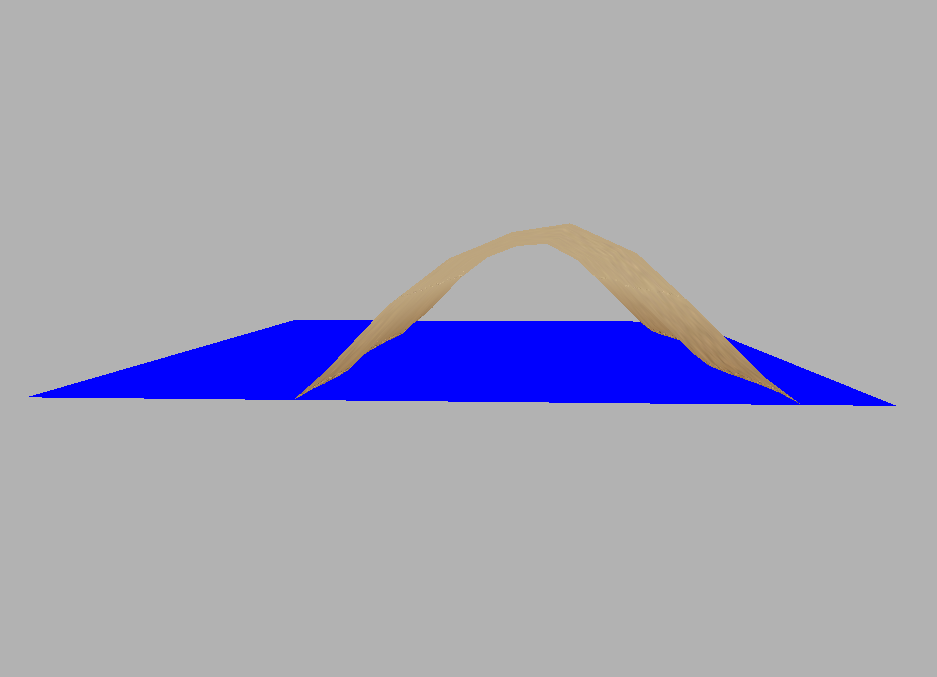
\includegraphics[width=6.3cm]{images/Water1.png}}}%
	\qquad
	\subfloat[\centering Clipping the above part.]{{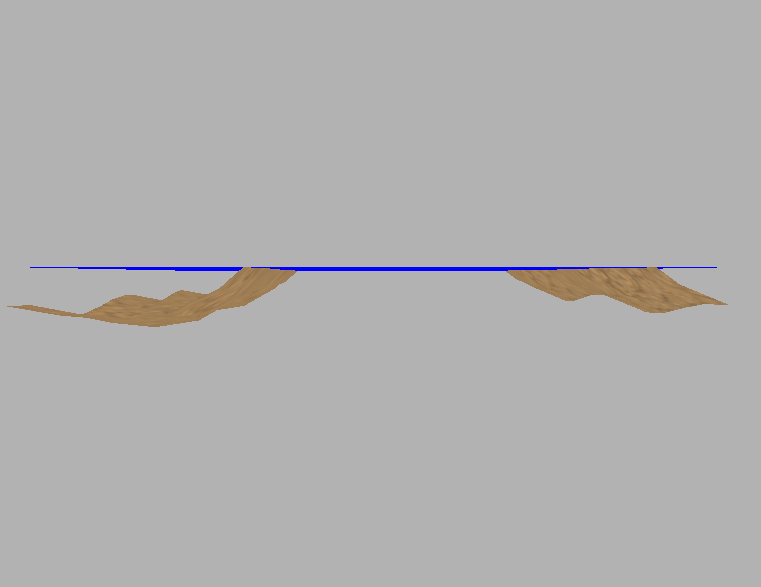
\includegraphics[width=6.3cm]{images/Water2.png} }}%
	\caption{}
\end{figure}

\subsection{Projective texture mapping}
To apply the texture to the plane, I used \textbf{projective texture mapping} that is a texture mapping method that allows you to project a textured image onto a scene. I needed to find the correct UV coordinate and for that I just found the screen space coordinate on the water coordinates and I can use those exactly to sample the texture. Basically I need to calculate the normalized device coordinates and I can do it using the perspective division. I just need to divide the clip space component (projection matrix * view matrix * model matrix * position) into its \textbf{W} component and then divide by 2 and add 0.5 to find the correct coordinate system .

\begin{equation}
newCoord = vec2(clipspace.xy / clipspace.w) 2.0 + 0.5)		
\end{equation}

\noindent
Now I can sample the refraction and the reflection by using the X and Y components as texture coordinates.
I also need to mention that the rendering for the reflection texture is done with the camera reversed and shifted slightly down to give the reflection effect. On the other hand, no changes are applied to refraction rendering.

\newpage

\begin{figure}[hbt!]
	\centering
	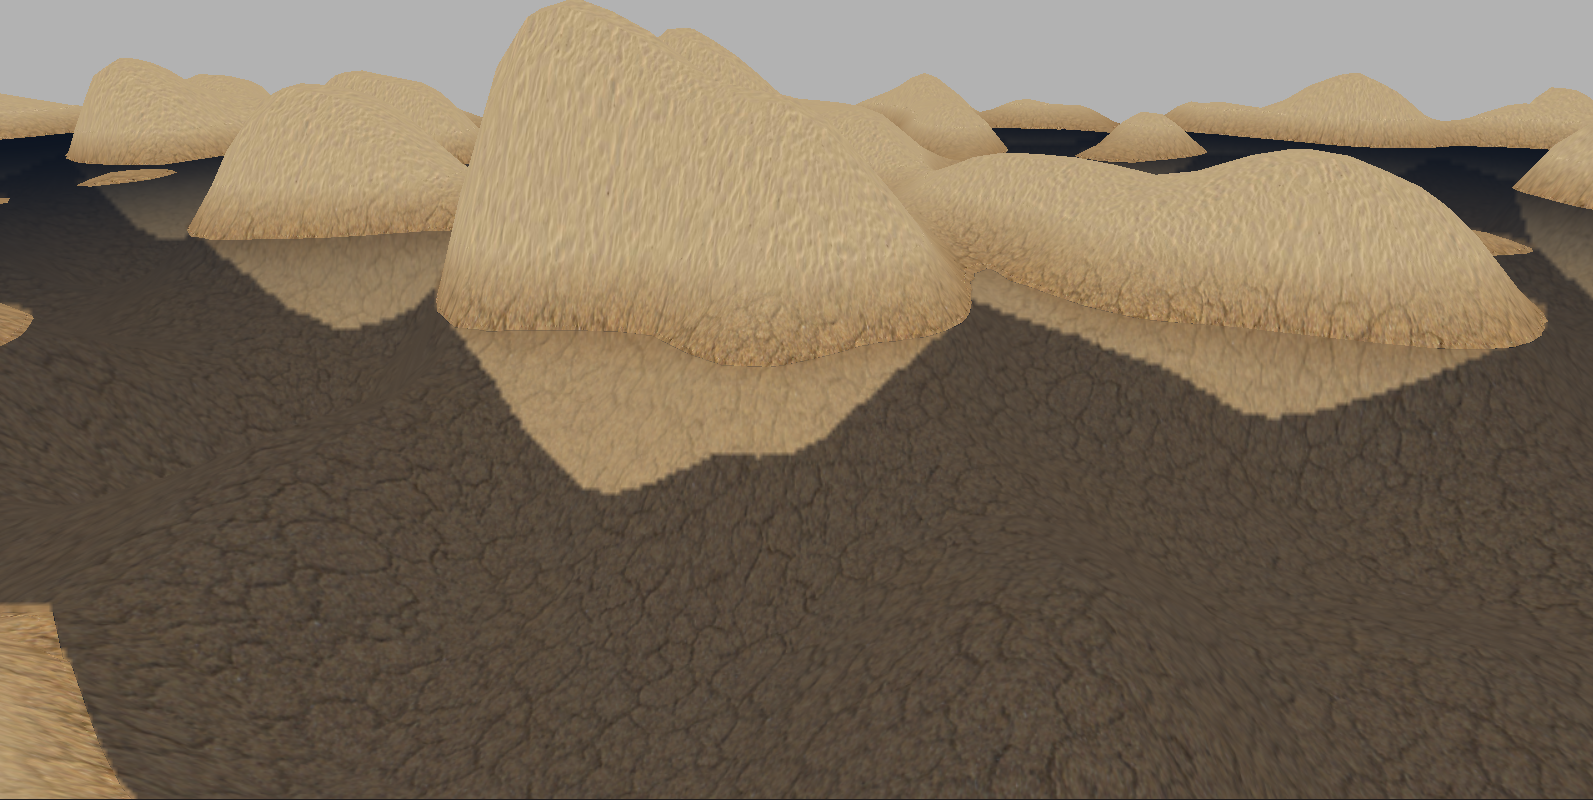
\includegraphics[width= 1
	\textwidth]{images/Water3.png}
	\caption{Reflection and Refraction texture mixed.}
\end{figure} 

\subsection{DuDv Maps}
To create a more realistic water, I used a particular texture to distort the water.

\begin{figure}[hbt!]
	\centering
	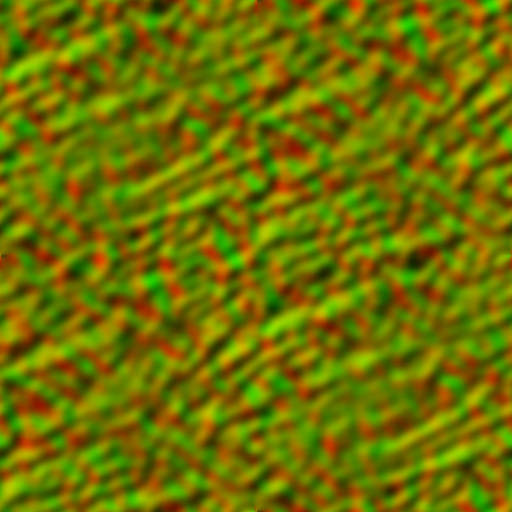
\includegraphics[width= 0.5
	\textwidth]{../textures/plane/waterDUDV.png}
	\caption{DuDv texture.}
\end{figure} 

\noindent
Basically, I try this new texture and used these coordinates to change the value of the previously calculated texture coordinates, in the x component and in the y component. To change the coordinates over time, I create a uniform variable called waterMovement to change the position of the coordinates at each frame. Since the value of our dudv texture is always positive, I applied a conversion to create value from -1 and 1, multiplied by 2 and subtracted 1. After adding the distortion, I clamped the result to have a value between 0 and 1.

\begin{figure}[hbt!]
	\centering
	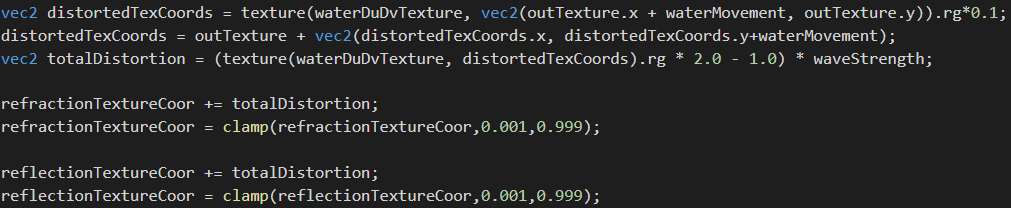
\includegraphics[width= 1
	\textwidth]{images/TextDist.png}
	\caption{\textbf{waterShader.frag} distortion part.}
\end{figure}

\begin{figure}[hbt!]
	\centering
	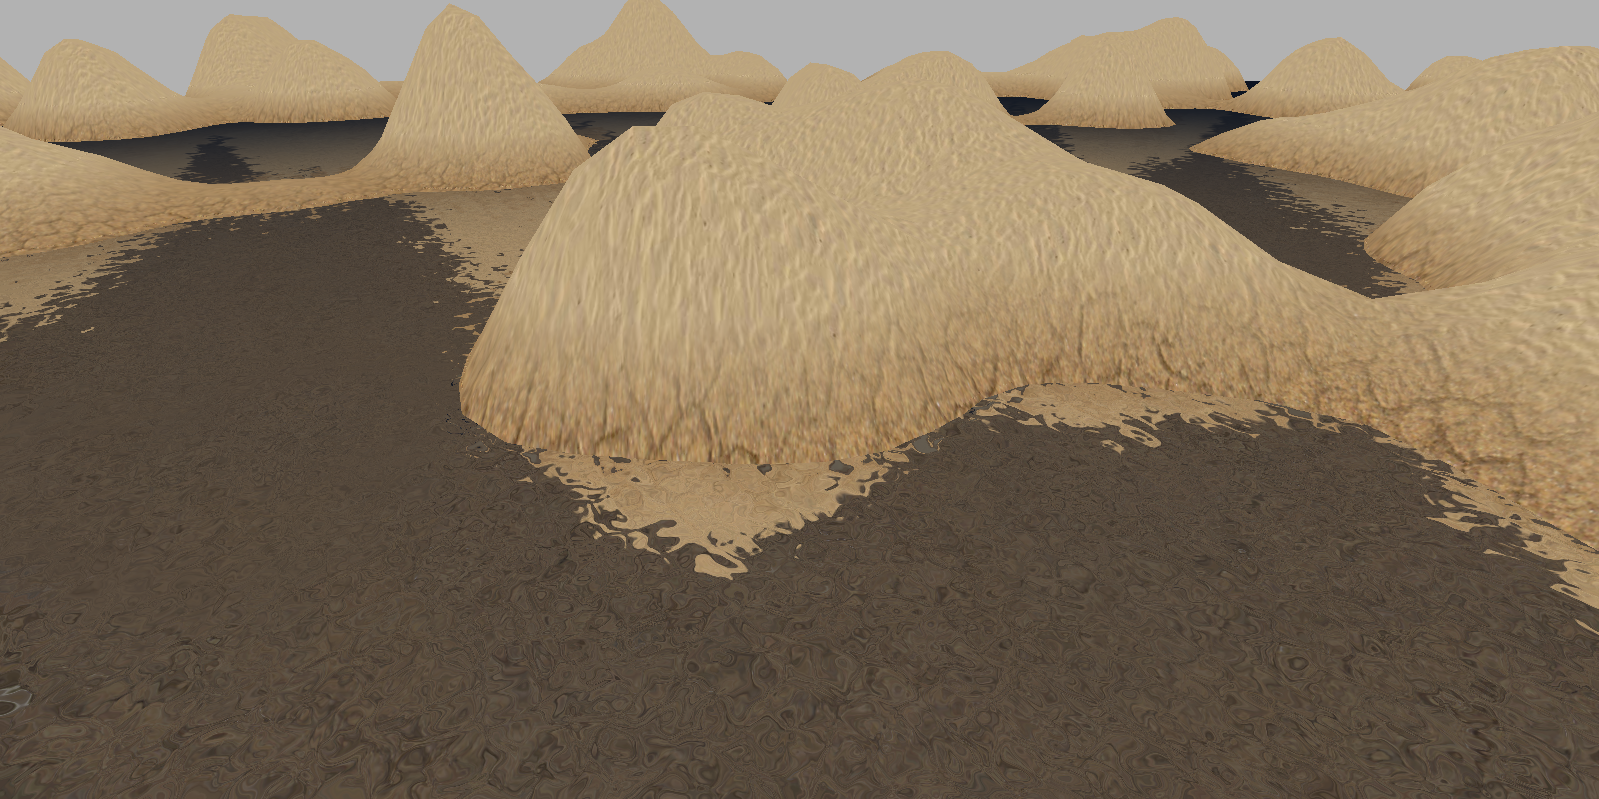
\includegraphics[width= 1
	\textwidth]{images/Water4.png}
	\caption{Water distortion.}
	\label{fig::distortion}
\end{figure}

\subsection{Normal map}
I want to simulate a light effect on the surface of the water. To do this I used a normal map which is similar to the dudv map above. 

\newpage

\begin{figure}[hbt!]
	\centering
	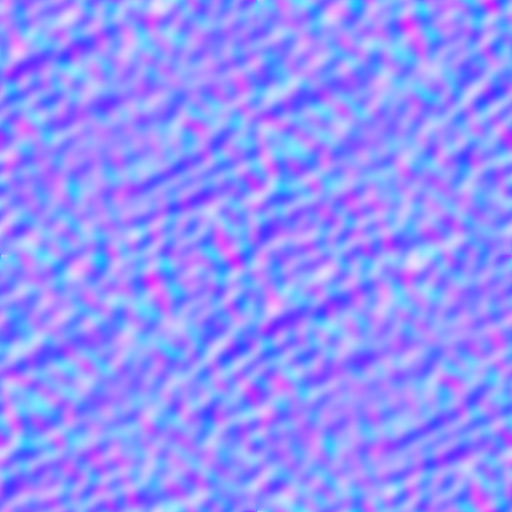
\includegraphics[width= 0.5
	\textwidth]{../textures/plane/normalMap.png}
	\caption{Normal texture.}
\end{figure} 

\noindent
In the shader, after sampling the texture, I calculated the normal vector using the red component for the X, the blue component for the Y and the green component for the Z. We want the Y component to always be positive, while the X and Z they can also be negative. So we multiplied the two coordinates by 2 and subtracted by 1 as we did before. After that I normalized the vectors.

\begin{equation}
\text{vec3 normal} = vec3(normalMap.r * 2 - 1, normalMap.b, normalMap.g * 2 - 1)		
\end{equation}

\noindent
Next I passed as uniform the position of the camera, the position of the light and I added a few more parameters to create the specular lighting on the water like \textbf{shineDamper} to determine the distance from where the camera will see any difference in the brightness of the surface and \textbf{reflectivity} which determined the amount of reflected light.
Then I calculated the vector from the light to the vertex using the world position (model * position) and the vector from the world position to the camera.

\begin{equation}
\text{vec3 fromLightVector} = normalize(WorldPosition - lightPos);
\end{equation}

\begin{equation}
\text{vec3 viewVector} = normalize(cameraPos - WorldPosition);
\end{equation}

\noindent
Now I can first calculate the reflection of \textbf{fromLightVector} with the normal, then calculate the dot product of \textbf {viewVector} and the reflected light to understand how bright the surface will be at that point. After that we had to use the pow function between the point product calculated earlier and the \textbf{shineDamper}. Finally, we can multiply the light colour (passed as uniform), the calculated specular illumination and the reflectivity.

\begin{figure}[hbt!]
	\centering
	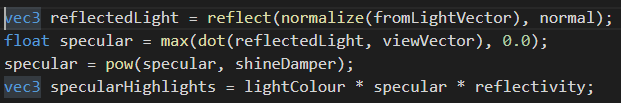
\includegraphics[width= 1
	\textwidth]{images/Light.png}
	\caption{Specular lighting code.}
	\label{fig::highlights}
\end{figure} 

\begin{figure}[hbt!]
	\centering
	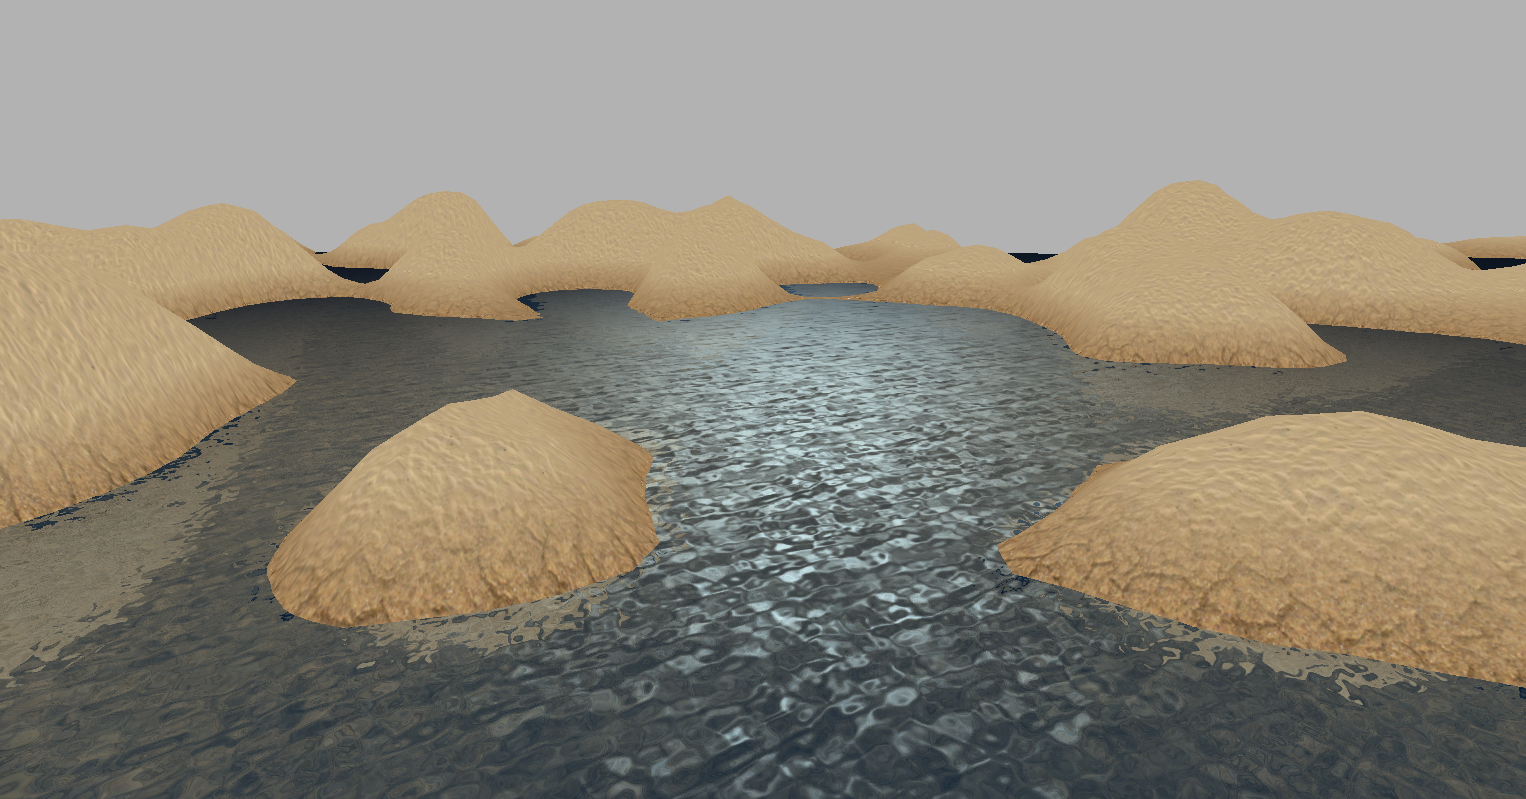
\includegraphics[width= 1
	\textwidth]{images/Water5.png}
	\caption{Specular lighting}
\end{figure} 

\subsection{Soft edges}
There is one last problem to be solved and it is caused by the distortion, in fact, there are rendered parts that should not be in the water.

\newpage

\begin{figure}[hbt!]
	\centering
	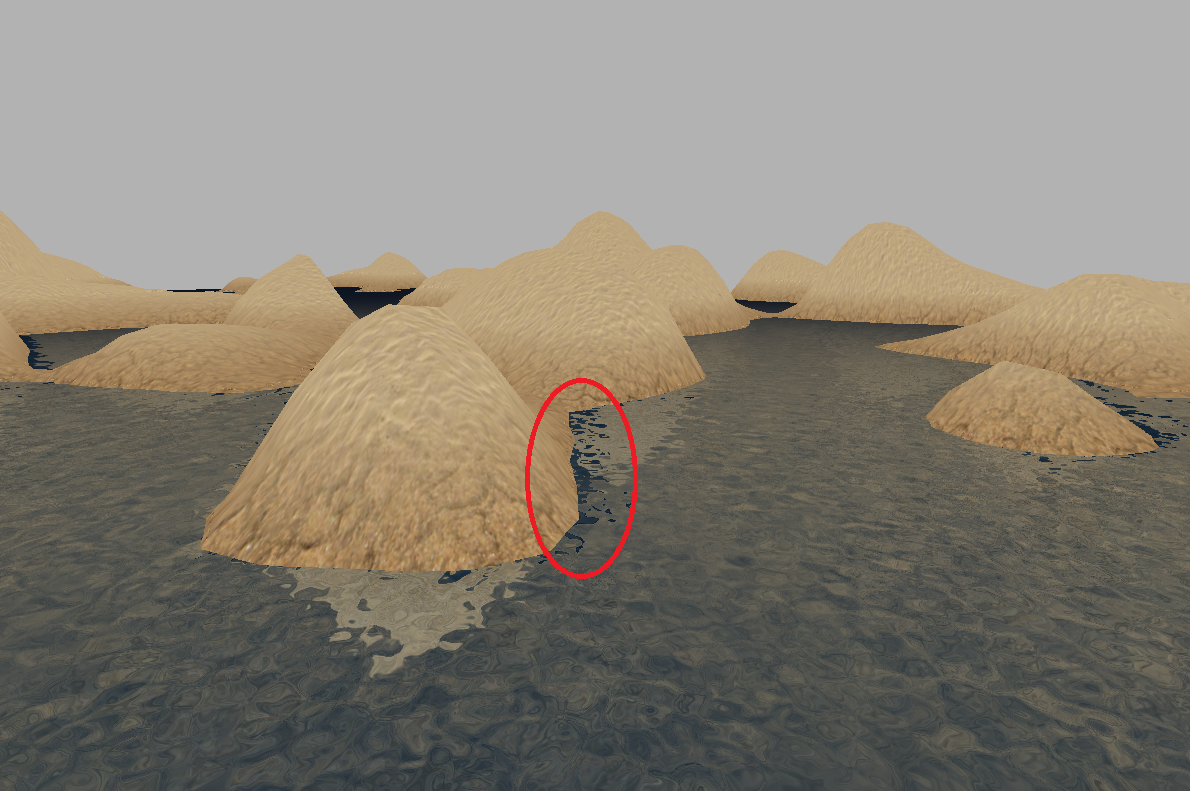
\includegraphics[width= 0.9
	\textwidth]{images/Water6.png}
	\caption{Picture that shows the problem}
\end{figure} 

\noindent
I want to calculate the distance between the bottom of the water and the water plane to the camera in the shader.

\begin{figure}[hbt!]
	\centering
	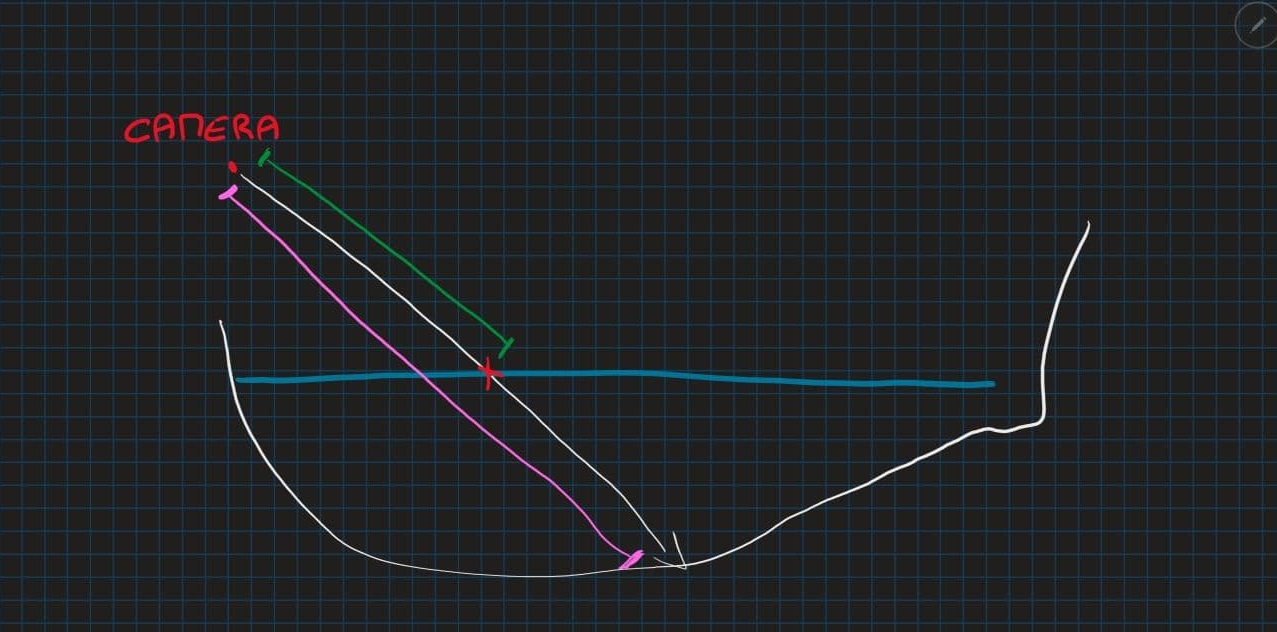
\includegraphics[width= 0.9
	\textwidth]{images/Water7.jpg}
	\caption{We want the subtraction between pink line and green line}
\end{figure} 

\noindent
To calculate the distance from the bottom of the water I will use the texture of the refractive depth calculated in the FBO. However, the \textbf{r} component of the depth texture gives us a value between 0 and 1. To convert it to a distance I used a formula that uses the far and near plane.
To calculate the distance from the plane I can use an OpenGl variable called \textbf{gl\textunderscore FragCoord}, then take the Z component that gives us the depth of this fragment and then apply the same formula as above. Finally I subtract the two values.

\begin{figure}[hbt!]
	\centering
	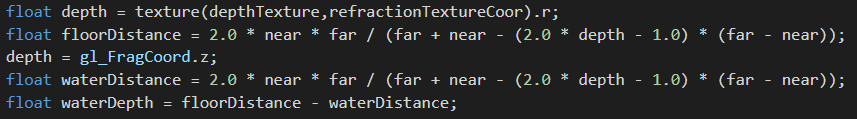
\includegraphics[width= 1
	\textwidth]{images/Water8.png}
	\caption{Code of the above passage.}
\end{figure} 

\begin{figure}[hbt!]
	\centering
	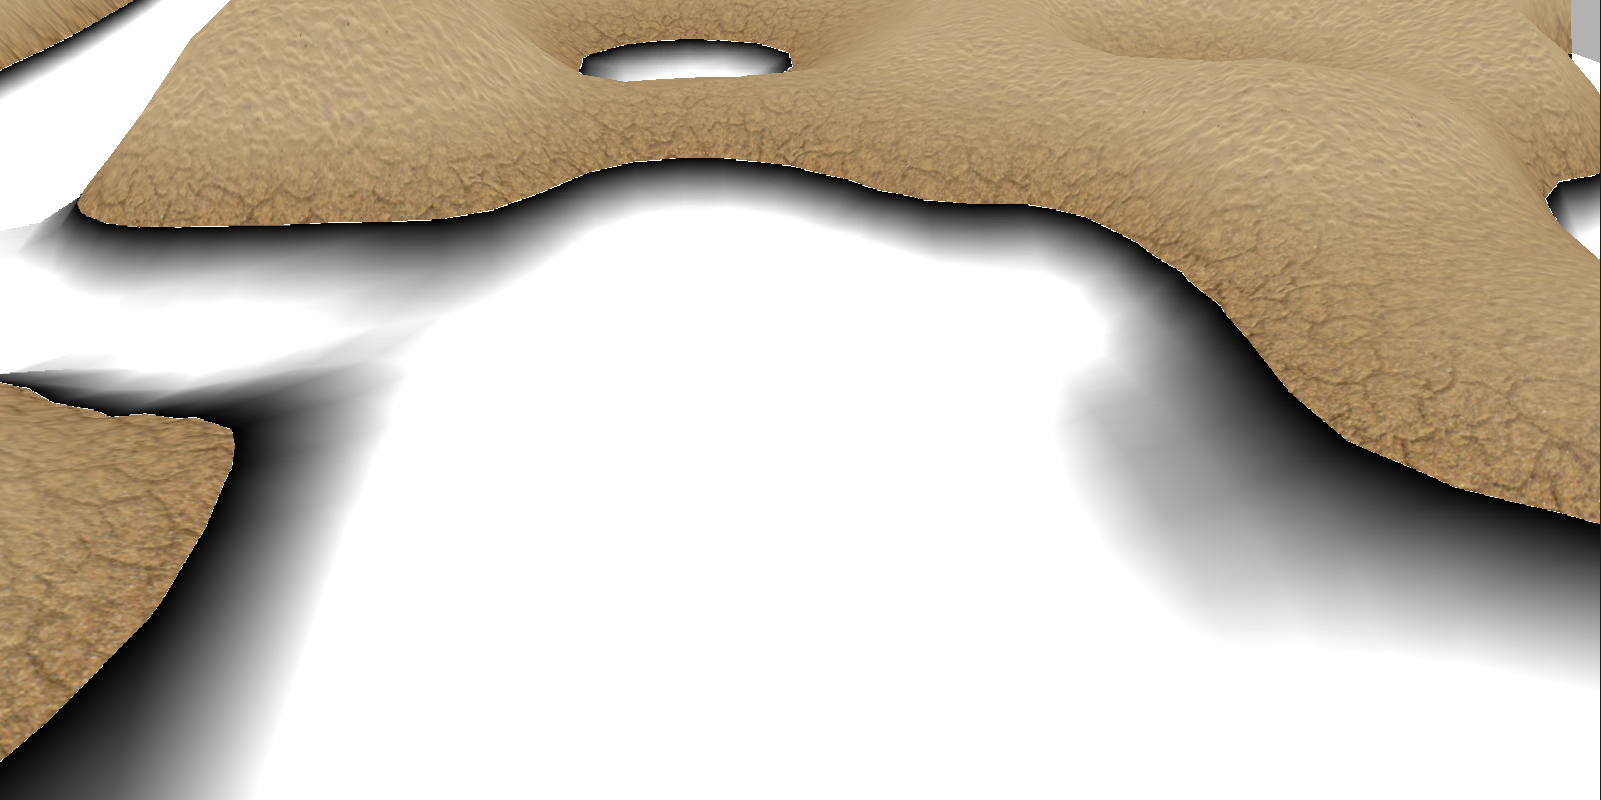
\includegraphics[width= 1
	\textwidth]{images/Water9.png}
	\caption{Water depth values applied in the water.}
\end{figure}

\noindent
Now we want to use this information to change the water near the edges. When the depth value is 0, the water is transparent. So the closer you get to the value 1, the less transparent the water is. After the value 1 there is no transparency.
Basically I just need to clamp my water depth (divided by a factor that determines how long the transition from 0 to 1 takes) and multiply it by the \textbf{totalDistortion} value in the figure \ref {fig :: distortion} and the value \textbf{specularHighlights} in figure \ref {fig :: highlights}.

\newpage

\begin{figure}[hbt!]
	\centering
	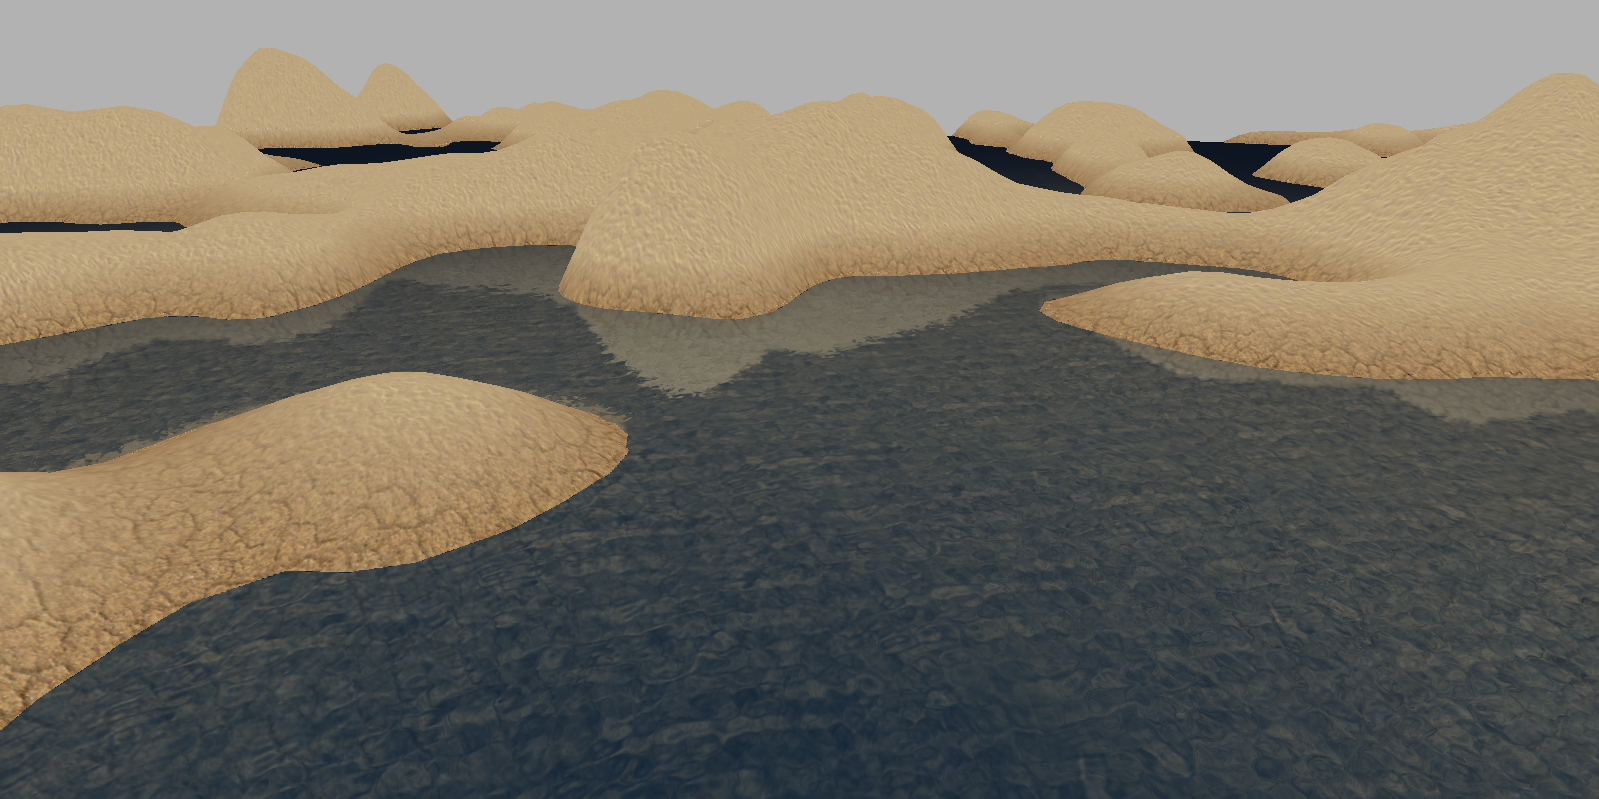
\includegraphics[width= 1
	\textwidth]{images/Water10.png}
	\caption{Water result after all stages.}
\end{figure}

\section{Cube Map}
I used a cube map to create the sky. One of the images I choose, contains moon to give the illusion that the light comes from there (the light source is indeed in the same direction).

\begin{figure}[hbt!]
	\centering
	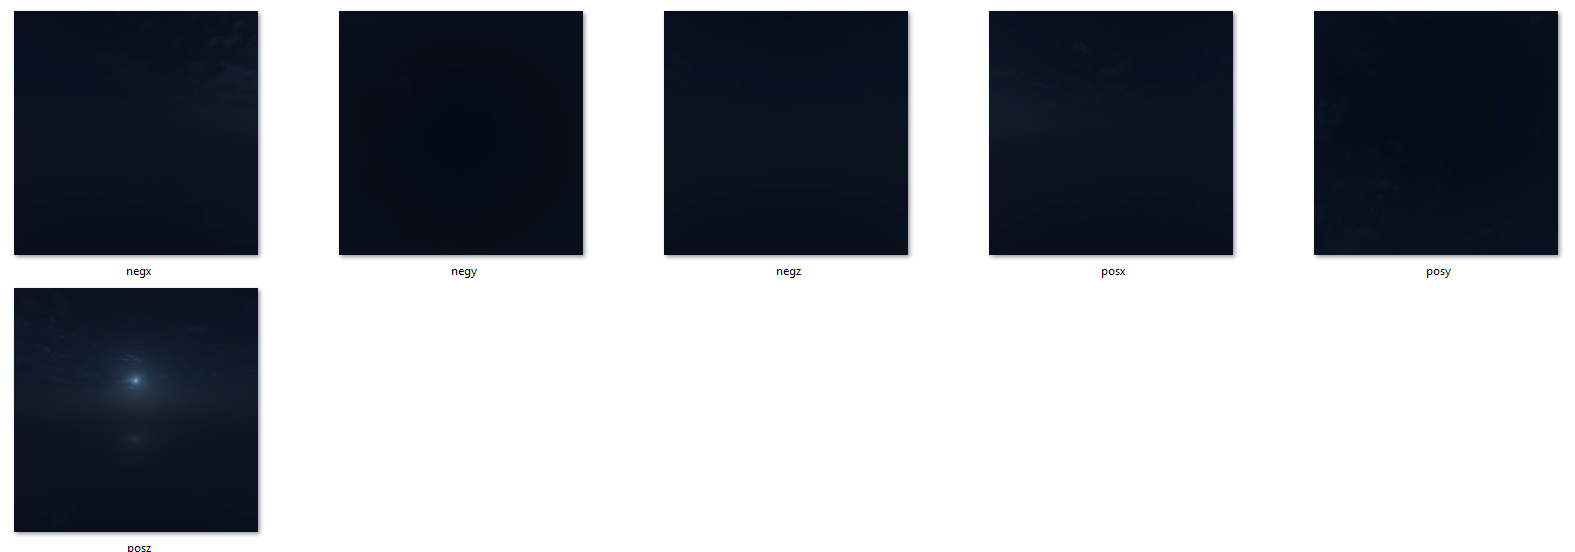
\includegraphics[width= 1
	\textwidth]{images/Sky.png}
	\caption{Images used for the cube map.}
\end{figure}

\newpage

\begin{figure}[hbt!]
\centering
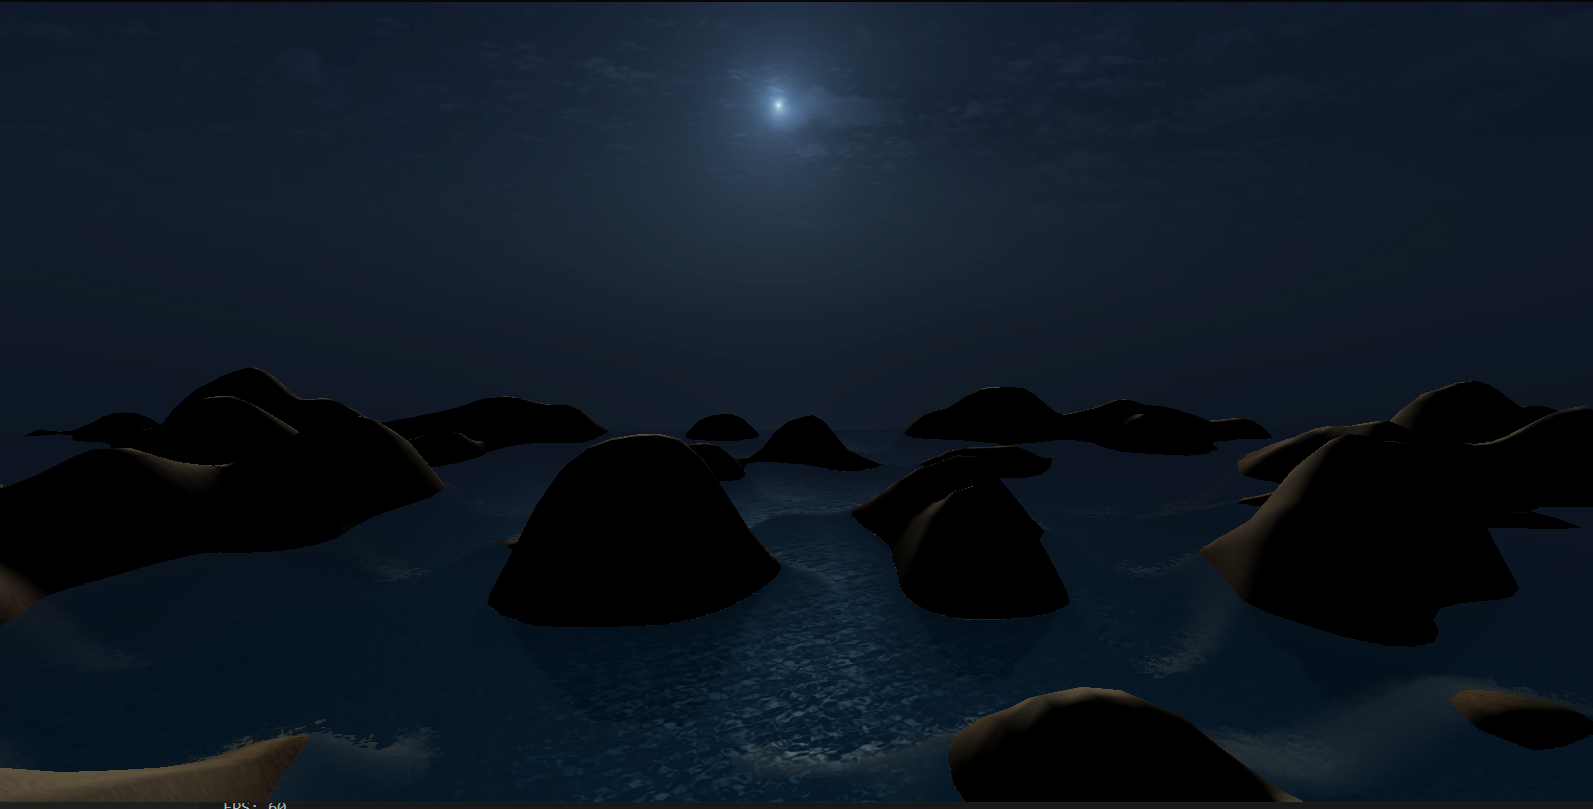
\includegraphics[width= 1
\textwidth]{images/Sky2.png}
\caption{Cube map applied.}
\end{figure}

\subsection{Fog}
Right now I can see the cells movement. To avoid this I need to create a Fog.